In this section, the results of simulations performed within this work are presented. Due to the limited space, we decided to attach figures only for the beams focused down to $ w_0 = 2.0 \ \mu\mathrm{m} $ and $ w_0 = 0.5 \ \mu\mathrm{m} $. These represent the cases of the focal spot larger than the center laser wavelength and the focal spot of a sub-wavelength level (tight-focusing). Nevertheless, the results of simulations for other focal spot sizes are compared and briefly discussed as well. In spite of the fact that in terms of physical relevance it would be more proper to compare the results of simulations with constant beam energies, they are discussed here only very briefly, because it is too difficult to recognize and distinguish only the effects of the focal spot size on the laser-matter interaction results.

First, the results have been analyzed in terms of the laser energy absorption efficiency. The comparison of the total laser light absorption in plasma for all performed simulations is shown in the table \ref{table:2}. It might be clearly seen that there is no significant difference between the absorption rates for the simulations where the beam is focused to a focal spot larger than the center laser wavelength whilst its peak intensity remains constant. On the other hand, in the case of the sub-wavelength focus, the rate of the energy absorption sharply increases. The ratio between the absorption of the beam focused to $ w_0 = 1.0 \ \mu\mathrm{m} $ and $ w_0 = 0.5 \ \mu\mathrm{m} $ is $ 1.7 $ in the case of the laser intensity $ I = 10^{20} \ \mathrm{W/cm^2} $ and $ 1.34 $ in the case of the intensity $ I = 10^{21} \ \mathrm{W/cm^2} $.

\begingroup
\renewcommand*{\arraystretch}{1.5}
\begin{table}[h!]
	\centering
	{\footnotesize
	\begin{tabular}{c | c | c | c}
		\multirow{2}{*}{$ w_0 $ [$ \mu\mathrm{m} $]} & \multicolumn{3}{c}{Total absorption of laser energy [\%]} \\ \cline{2-4}
		& const. $ E \approx 30 \ \mathrm{mJ} $ & const. $ I = 10^{20} \ \mathrm{W/cm^2} $ & const. $ I = 10^{21} \ \mathrm{W/cm^2} $ \\ \hline \hline
		0.5 & 20.12 & 16.23 & 31.77 \\ \hline
		1.0 & 9.59 & 9.59 & 23.76 \\ \hline
		2.0 & 5.27 & 8.26 & 23.82 \\ \hline
		4.0 & 3.49 & 8.29 & 23.71 \\
	\end{tabular}}
	\caption{Total laser energy absorption in plasma for several different sizes of the focal spot and different laser intensities.}
	\label{table:2}
\end{table}
\endgroup

\begingroup
\renewcommand*{\arraystretch}{1.5}
\begin{table}[h!]
	\centering
	{\footnotesize
	\begin{tabular}{c | c | c }
		$ w_0 $ [$ \mu\mathrm{m} $]	& $ k_B T $ of hot electrons [MeV] & maximum energy of ions [MeV] \\ \hline \hline
		0.5 & 0.93 & 4.73 \\ \hline
		1.0 & 0.64 & 1.71 \\ \hline
		2.0 & 0.32 & 0.74 \\ \hline
		4.0 & 0.16 & 0.43 \\
	\end{tabular}}
	\caption{Temperature of hot electrons estimated by fitting the energy distributions at the time $ t = 100 \ \mathrm{fs} $ by Maxwellian functions and the maximum ion energy at the time $ t = 150 \ \mathrm{fs} $ for the laser beam with constant energy $ E \approx 30 \ \mathrm{mJ} $ and several different sizes of the focal spot.}
	\label{table:3}
\end{table}
\endgroup

\floatsetup[figure]{style=plain, subcapbesideposition=top}
\begin{figure}[h!]
	\centering
	\sidesubfloat[]{{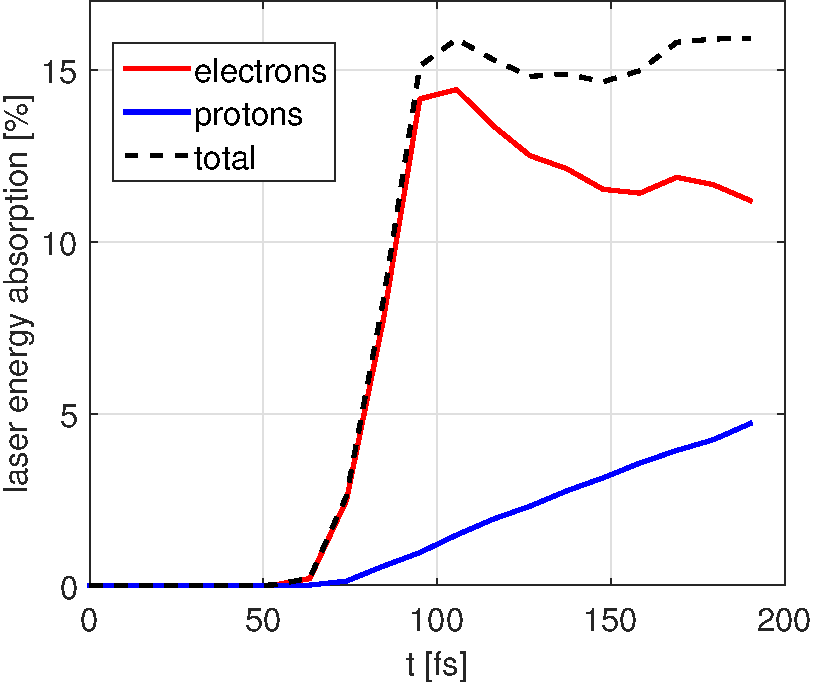
\includegraphics[width=0.45\linewidth]{./img/results/i1e20/05/absorp.pdf}}}
	\sidesubfloat[]{{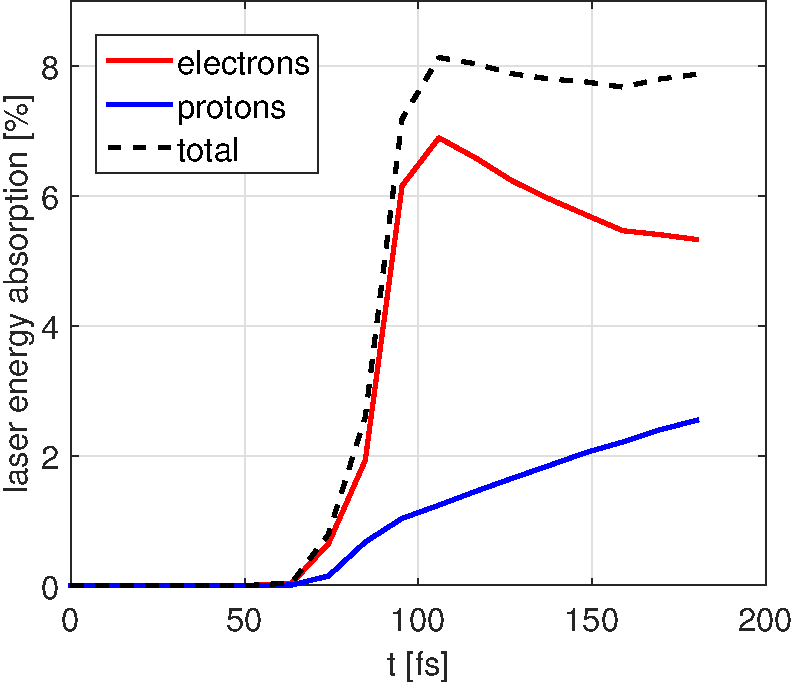
\includegraphics[width=0.45\linewidth]{./img/results/i1e20/2/absorp.pdf}}}\\
	\sidesubfloat[]{{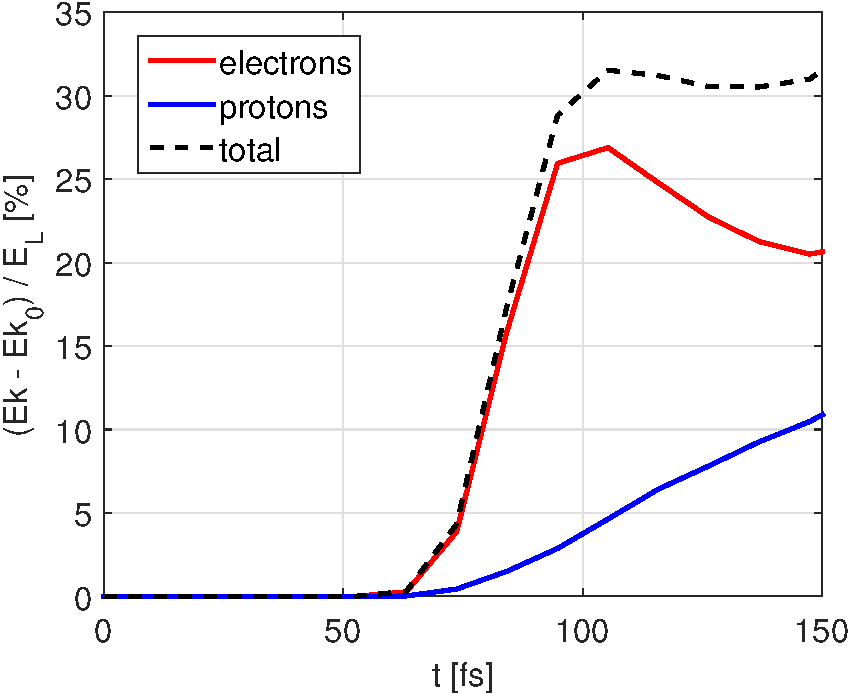
\includegraphics[width=0.45\linewidth]{./img/results/i1e21/05/absorp.pdf}}}
	\sidesubfloat[]{{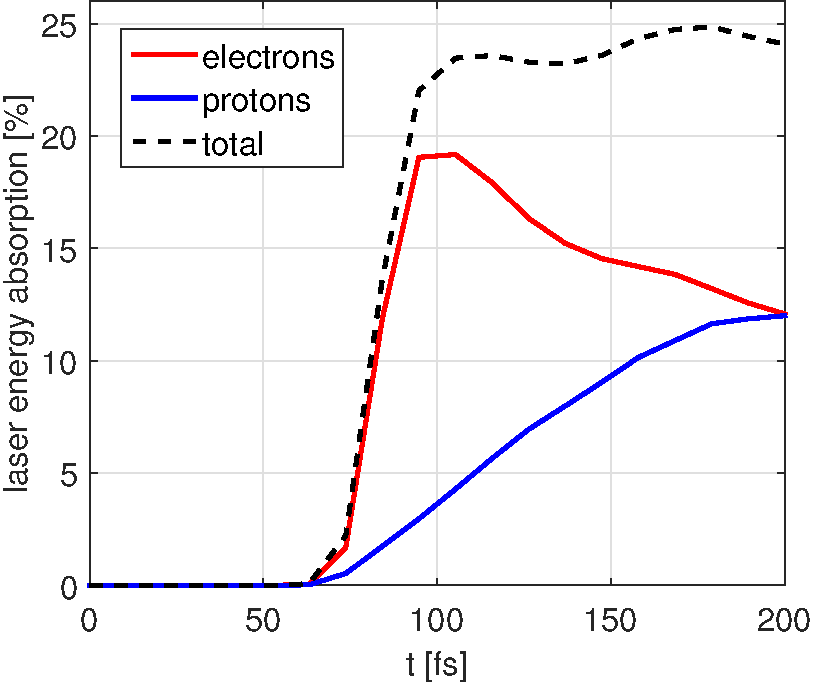
\includegraphics[width=0.45\linewidth]{./img/results/i1e21/2/absorp.pdf}}}
	\caption{The kinetic energy $ E_k $ of particles ($ E_{k0} $ denotes the initial kinetic energy of particles) normalized to the laser pulse energy $ E_L $ in time for the case of simulations with the laser intensity $ I = 10^{20} \ \mathrm{W/cm^2} $ and with the beam waist \textbf{(a)} $ w_0 = 0.5 \ \mu\mathrm{m} $, \textbf{(b)} $ w_0 = 2.0 \ \mu\mathrm{m} $ and for the case of simulations with the laser intensity $ I = 10^{21} \ \mathrm{W/cm^2} $ and with the beam waist \textbf{(c)} $ w_0 = 0.5 \ \mu\mathrm{m} $, \textbf{(d)} $ w_0 = 2.0 \ \mu\mathrm{m} $.}
	\label{fig:10}
\end{figure}

\floatsetup[figure]{style=plain, subcapbesideposition=top}
\begin{figure}[h!]
	\centering
	\sidesubfloat[]{{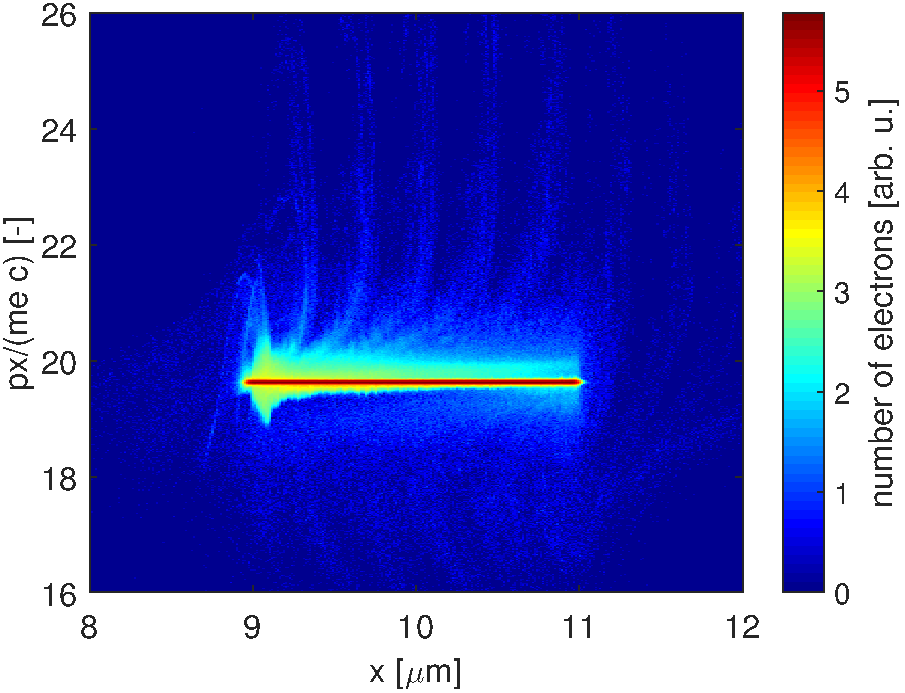
\includegraphics[width=0.45\linewidth]{./img/results/i1e20/05/x_px.pdf}}}
	\sidesubfloat[]{{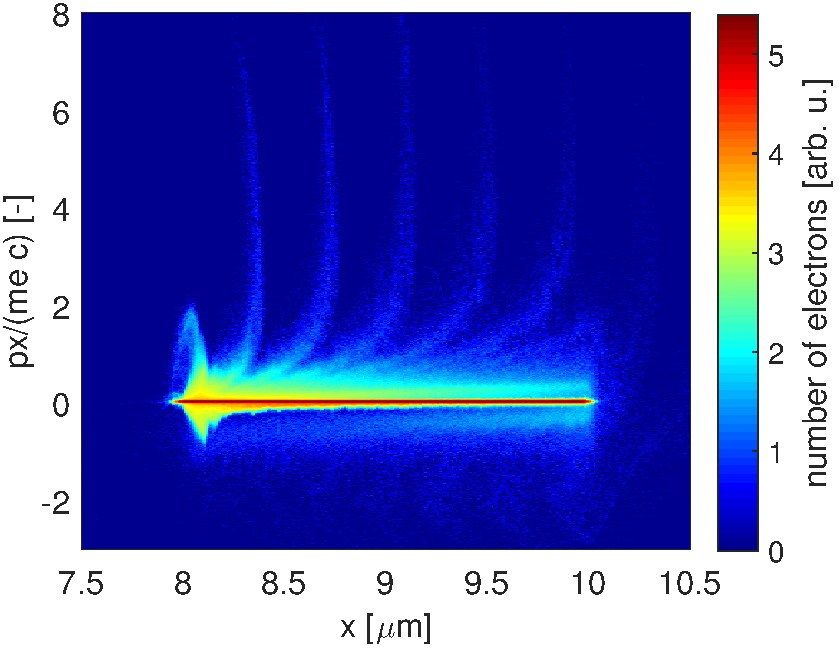
\includegraphics[width=0.45\linewidth]{./img/results/i1e20/2/x_px.pdf}}}\\
	\sidesubfloat[]{{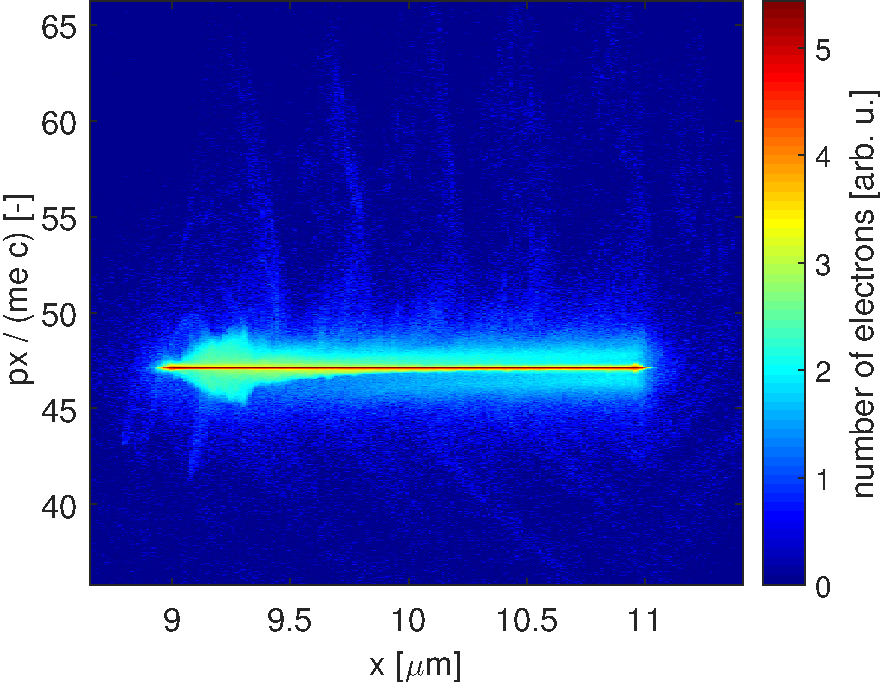
\includegraphics[width=0.45\linewidth]{./img/results/i1e21/05/x_px.pdf}}}
	\sidesubfloat[]{{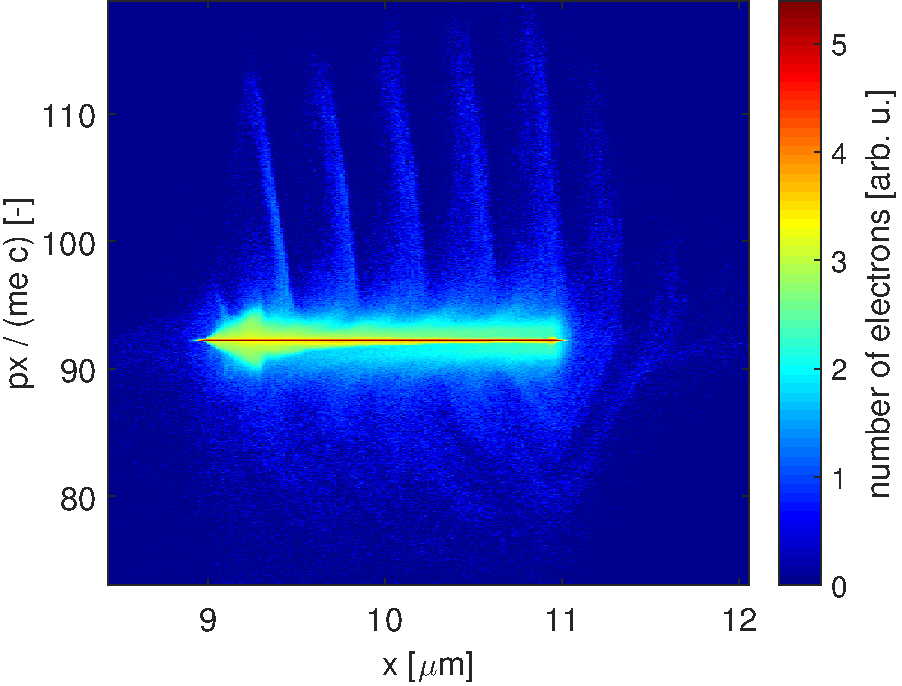
\includegraphics[width=0.45\linewidth]{./img/results/i1e21/2/x_px.pdf}}}
	\caption{The phase space of the parallel component of the momentum ($ p_x $) and the x-coordinate of all electrons in the simulation domain at the time $ t = 100 \ \mathrm{fs} $ for the case of simulations with the laser intensity $ I = 10^{20} \ \mathrm{W/cm^2} $ and with the beam waist \textbf{(a)} $ w_0 = 0.5 \ \mu\mathrm{m} $, \textbf{(b)} $ w_0 = 2.0 \ \mu\mathrm{m} $ and for the case of simulations with the laser intensity $ I = 10^{21} \ \mathrm{W/cm^2} $ and with the beam waist \textbf{(c)} $ w_0 = 0.5 \ \mu\mathrm{m} $, \textbf{(d)} $ w_0 = 2.0 \ \mu\mathrm{m} $. The color scales are logarithmic and the units are arbitrary, but the same for all sub-figures.}
	\label{fig:11}
\end{figure}

The simulations with constant laser beam energy result in increasing hot electron temperature and maximum ion energy as the focal spot size decreases as can be seen from the table \ref{table:3}. One would expect a much weaker scaling of the hot electron temperature due to the $ \vec{J} \times \vec{B} $ heating \cite{Gibbon2005} and of the maximum proton energy in the TNSA regime with the laser intensity ($ \sim \sqrt{I} $) \cite{Wilks1992, Zeil2010, Fuchs2006}. However, the absorption rates for the laser beam with a given waist strongly depend on the laser intensity at focus as can be seen in the table \ref{table:2} comparing the last two columns. Therefore, to better understand the dependency of the energy absorption on the size of the focal spot, it is better to further study the results of laser-matter interaction for the laser beams with constant intensities.

\floatsetup[figure]{style=plain, subcapbesideposition=top}
\begin{figure}[h!]
	\centering
	\sidesubfloat[]{{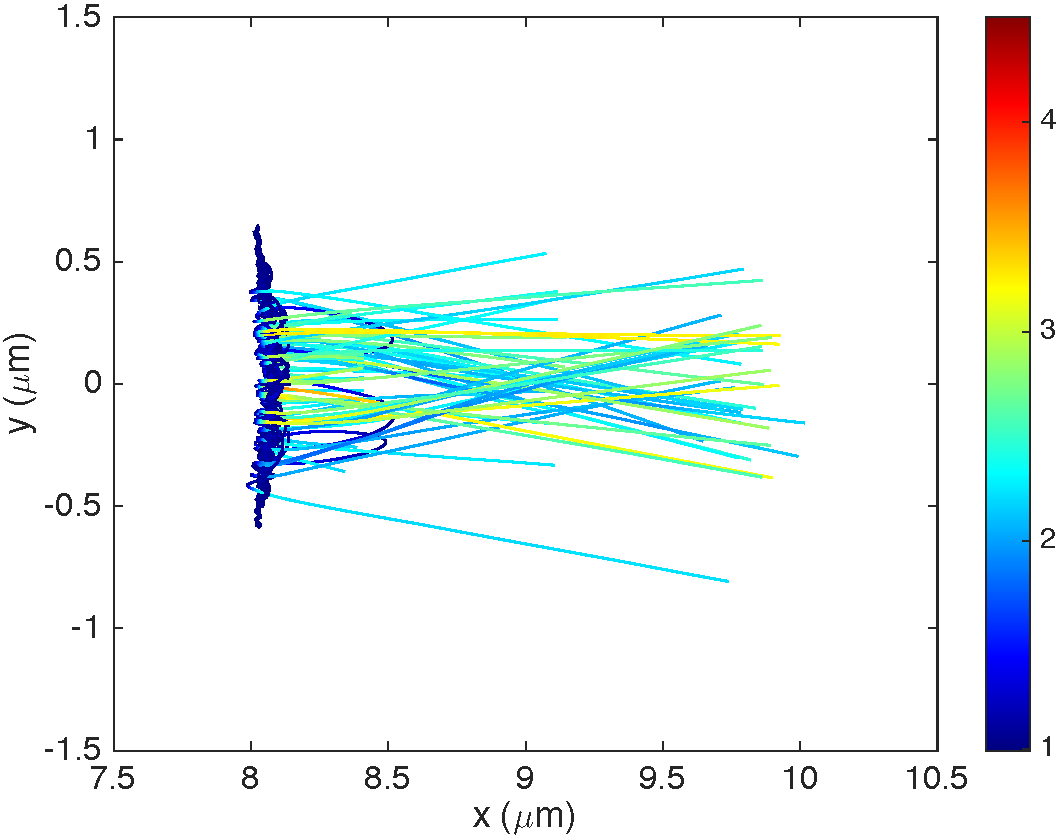
\includegraphics[width=0.4\linewidth]{./img/results/i1e20/05/traj_1.pdf}}}
	\sidesubfloat[]{{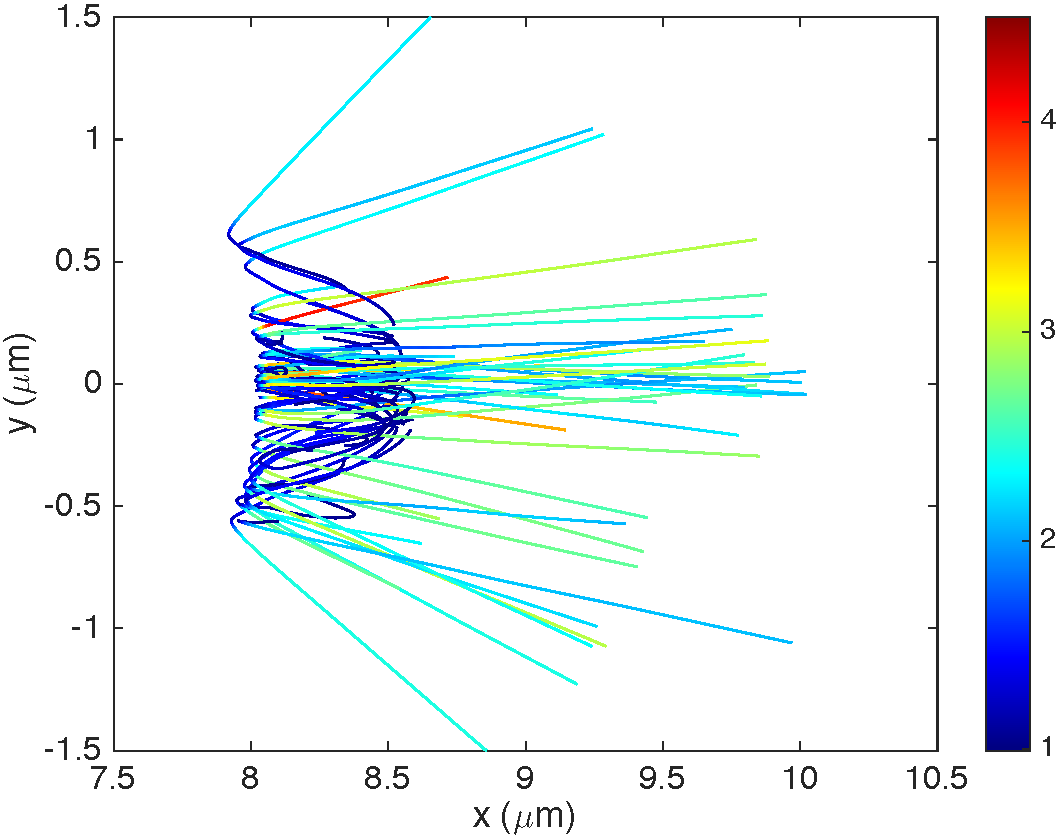
\includegraphics[width=0.4\linewidth]{./img/results/i1e20/05/traj_2.pdf}}}\\[2mm]
	\sidesubfloat[]{{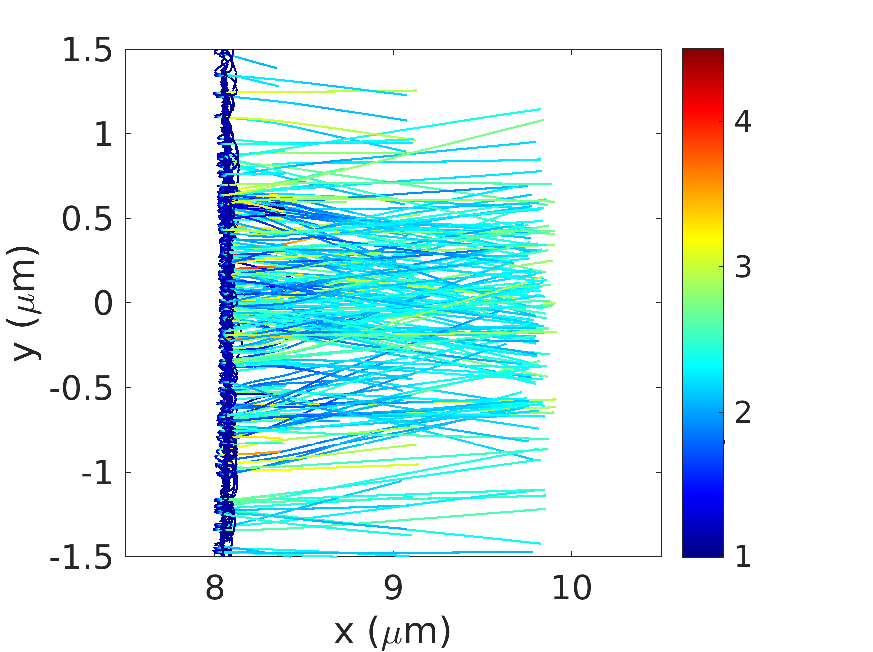
\includegraphics[width=0.4\linewidth]{./img/results/i1e20/2/traj_1.pdf}}}
	\sidesubfloat[]{{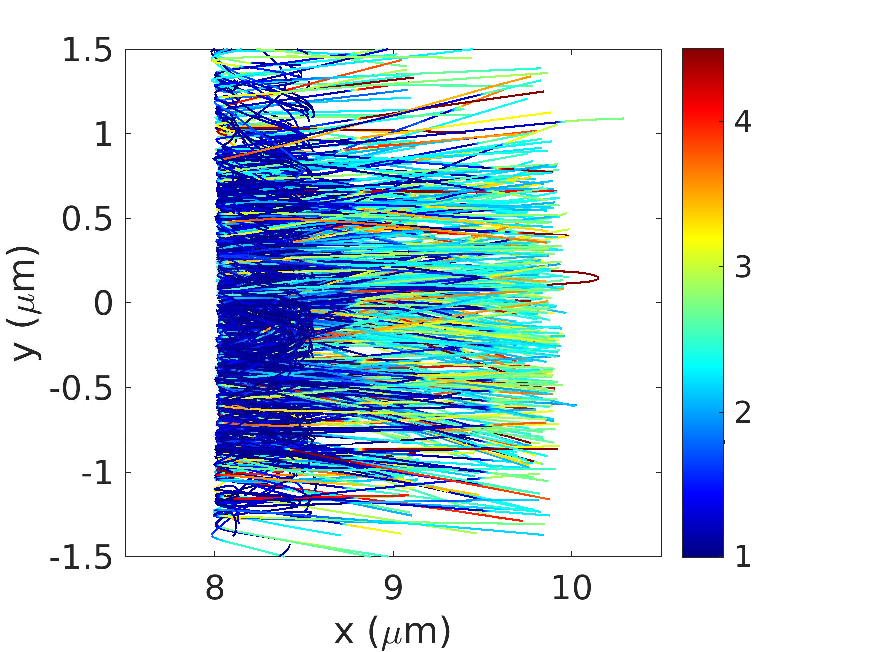
\includegraphics[width=0.4\linewidth]{./img/results/i1e20/2/traj_2.pdf}}}
	\caption{Two types of trajectories of randomly chosen electron samples for the case of simulations with the laser intensity $ I = 10^{20} \ \mathrm{W/cm^2} $ and with the beam waist \textbf{(a), (b)} $ w_0 = 0.5 \ \mu\mathrm{m} $ and \textbf{(c), (d)} $ w_0 = 2.0 \ \mu\mathrm{m} $. The trajectories are colored according to the Lorentz $ \gamma $ factor of corresponding particles.}
	\label{fig:19}
\end{figure}

The temporal evolution of the kinetic energy of particles normalized to the laser pulse energy can be seen in the fig. \ref{fig:10}. The maximum kinetic energy of electrons occurs when the peak intensity reaches the target at the time $ t = 100 \ \mathrm{fs} $. Even before that, when the hot electron population becomes significant ($ \sim 80 \ \mathrm{fs} $) ion acceleration sets in. In the case of these intensities and the p-polarization, it is dominated by the TNSA processes closer described in the chapter 2. The plots indicate that as the focal spot size increases, the energy transfer to ions is faster. This may have two reasons. Either the electric field induced by the expanding hot electrons on the target surface is higher or it decays more slowly with time. Note that even if the absorption is lower for larger spot size, the amount of energy absorbed in the target is higher because of the four times higher laser energy. Nevertheless, to understand the energy transfer from hot electrons to ions, one has to identify the main plasma heating and energy absorption mechanisms.

\floatsetup[figure]{style=plain, subcapbesideposition=top}
\begin{figure}[h!]
	\centering
	\sidesubfloat[]{{\includegraphics[width=0.45\linewidth]{./img/results/i1e20/05/fpx.pdf}}}
	\sidesubfloat[]{{\includegraphics[width=0.45\linewidth]{./img/results/i1e20/05/fpy.pdf}}}\\
	\sidesubfloat[]{{\includegraphics[width=0.45\linewidth]{./img/results/i1e20/2/fpx.pdf}}}
	\sidesubfloat[]{{\includegraphics[width=0.45\linewidth]{./img/results/i1e20/2/fpy.pdf}}}
	\caption{The longitudinal ($ F_{\mathrm{p}, x} $) \textbf{(a)} and the transverse ($ F_{\mathrm{p}, y} $) \textbf{(b)} component of the ponderomotive force for the case of the laser beam with intensity $ I = 10^{20} \ \mathrm{W/cm^2} $ and the beam waist $ w_0 = 0.5 \ \mu\mathrm{m} $ propagating in vacuum. The longitudinal ($ F_{\mathrm{p}, x} $) \textbf{(c)} and the transverse ($ F_{\mathrm{p}, y} $) \textbf{(d)} component of the ponderomotive force for the case of the laser beam with intensity $ I = 10^{20} \ \mathrm{W/cm^2} $ and the beam waist $ w_0 = 2.0 \ \mu\mathrm{m} $ propagating in vacuum. The ponderomotive force has been calculated according to the non-relativistic formula \ref{2.5.1.11}.}
	\label{fig:21}
\end{figure}

It is expected that the dominating absorption mechanism is $ \vec{J} \times \vec{B} $ heating for the laser intensities used in the simulations. The phase space of the parallel component of the momentum and the x-coordinate of all electrons in the simulation domain at the time $ t = 100 \ \mathrm{fs} $ is shown in the fig. \ref{fig:11}. The bunches of hot electrons that are ejected twice per laser period due to the $ \vec{J} \times \vec{B} $ heating are more compact and clearly visible in the case of $ w_0 = 2.0 \ \mu\mathrm{m} $. The peak longitudinal momentum $ p_x \approx 8 \ m_{e} c $ in the case of the laser intensity $ I = 10^{20} \ \mathrm{W/cm^2} $ and $ p_x \approx 22 \ m_{e} c $ in the case of the intensity $ I = 10^{21} \ \mathrm{W/cm^2} $ independently of the focal spot size. On the other hand, the phase space looks similar in the region $ \abs{p_x} < 0.5 $ of non-relativistic hot electrons. The main difference is that the number of these hot electrons is higher for the larger spot size. Yet another qualitative difference can be observed, there is a significant cloud of hot electrons in front of the target for the smaller spot size which is missing for the larger one.

\floatsetup[figure]{style=plain, subcapbesideposition=top}
\begin{figure}[h!]
	\centering
	\sidesubfloat[]{{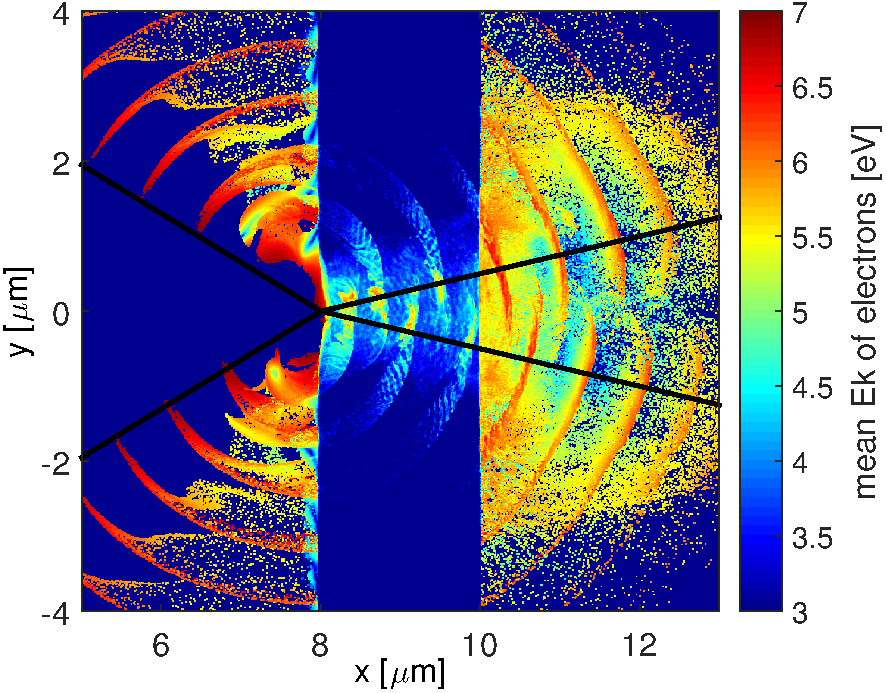
\includegraphics[width=0.45\linewidth]{./img/results/i1e21/05/ekbar_2.pdf}}}
	\sidesubfloat[]{{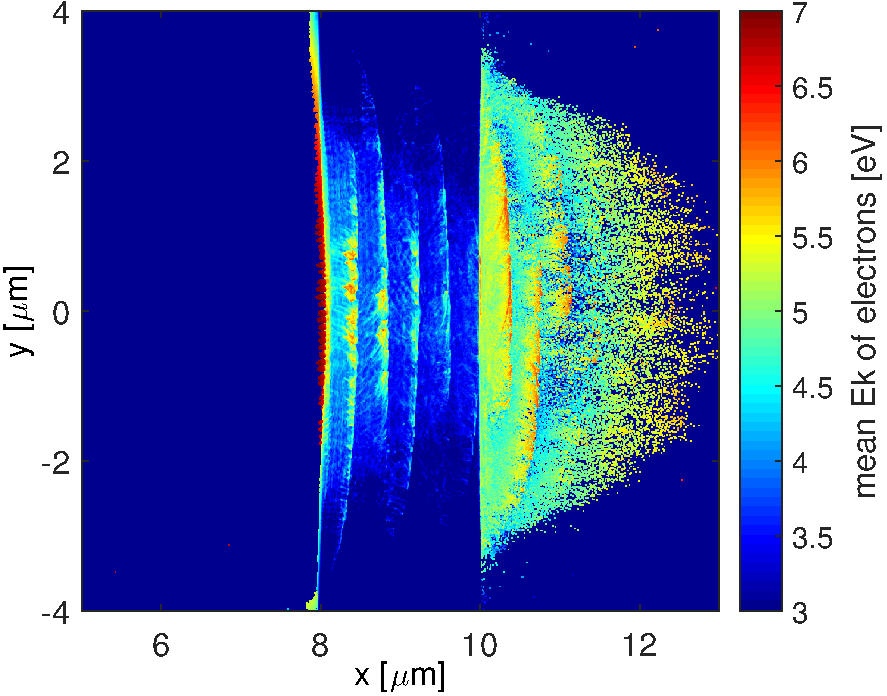
\includegraphics[width=0.45\linewidth]{./img/results/i1e21/2/ekbar_2.pdf}}}\\[2mm]
	\caption{The spatial distribution of the mean kinetic energy of electrons at the time $ t = 80 \ \mathrm{fs} $ for the case of simulations with the laser intensity $ I = 10^{21} \ \mathrm{W/cm^2} $ and with the beam waist \textbf{(a)} $ w_0 = 0.5 \ \mu\mathrm{m} $, \textbf{(b)} $ w_0 = 2.0 \ \mu\mathrm{m} $. The color scales are logarithmic.}
	\label{fig:17}
\end{figure}

For deeper understanding, it might be useful to track trajectories of hot electrons. The fig. \ref{fig:19} shows such trajectories for the laser intensity $ I = 10^{20} \ \mathrm{W/cm^2} $. These electrons are tracked during three laser periods around the peak laser intensity and we show a randomly chosen $ 10 \ \% $ of hot electrons that have the final $ \gamma $ factor at least two times higher than the initial one for this time interval. It turned out that most of the trajectories can be split up into two groups. The first type of trajectories corresponds to electrons that move along the front surface of the target towards the focal spot and in the vicinity of the focus, these electrons are pushed into the target by $ \vec{J} \times \vec{B} $ force (fig. \ref{fig:19}-a, \ref{fig:19}-c). The second type of trajectories corresponds to electrons that are initially inside the target, they come out to the target front surface as a return current and are pushed back to the plasma by $ \vec{J} \times \vec{B} $ force (fig. \ref{fig:19}-b, \ref{fig:19}-d). Note that there is a significant quantitative difference between the two focal spot sizes for both types of trajectories. In the case of $ w_0 = 0.5 \ \mu\mathrm{m} $, there is approximately $ 59 \ \% $ of electrons with the trajectories of the first type (fig. \ref{fig:19}-a) and $ 41 \ \% $ of the second type (fig. \ref{fig:19}-b). On the contrary, for the simulation of $ w_0 = 2.0 \ \mu\mathrm{m} $, there is about $ 22 \ \% $ of electrons with the trajectories of the first type (fig. \ref{fig:19}-c) and $ 78 \ \% $ of the second type (fig. \ref{fig:19}-d). It also seems that the beam of accelerated electrons is more divergent in the case of the smaller spot size.

The electron trajectories are determined mainly by the field of incident laser pulse. In the fig. \ref{fig:21}, one can see the longitudinal and transverse components of the ponderomotive force for the laser beam with intensity $ I = 10^{20} \ \mathrm{W/cm^2} $ propagating in vacuum. The magnitude of longitudinal component is almost the same for both focal spot sizes (for the tight-focusing, the force is not plotted exactly at the time of the peak laser intensity due to the discrete time step), but the transverse component is approximately $ 3.5 $ times higher in the case of $ w_0 = 0.5 \ \mu\mathrm{m} $. The ratio of the transverse component of the ponderomotive force to the longitudinal component is approximately $ 0.31 $ in the case of $ w_0 = 0.5 \ \mu\mathrm{m} $ (fig. \ref{fig:21}-a, \ref{fig:21}-b) and $ 0.08 $ in the case of $ w_0 = 2.0 \ \mu\mathrm{m} $ (fig. \ref{fig:21}-c, \ref{fig:21}-d). Note that for the laser intensity $ I = 10^{21} \ \mathrm{W/cm^2} $, the values of ponderomotive force are one order of magnitude higher, but the ratios between longitudinal and transverse components remain identical.

The spatial distribution of the mean kinetic energy of electrons at the time $ t = 80 \ \mathrm{fs} $ is shown in the fig. \ref{fig:17}. The direction of electrons moving forward is given by the ratio of the transverse component of the ponderomotive force to the longitudinal component. In the case of $ w_0 = 0.5 \ \mu\mathrm{m} $, the angle (marked by a black line in the fig. \ref{fig:17}-a) is estimated to $ 17.4^{\circ} $, whilst in the case of $ w_0 = 2.0 \ \mu\mathrm{m} $ (fig. \ref{fig:17}-b), the angle is only $ 4.5^{\circ} $. In both cases, one may see the bunches of hot electrons that are ejected twice per laser period. In addition, in the case of $ w_0 = 0.5 \ \mu\mathrm{m} $, one may also clearly see the electrons that move backwards. Their movement is restricted by the incoming laser beam (the laser divergence angle is marked by a black line in front of the target in the fig. \ref{fig:17}-a).

\floatsetup[figure]{style=plain, subcapbesideposition=top}
\begin{figure}[h!]
	\centering
	\sidesubfloat[]{{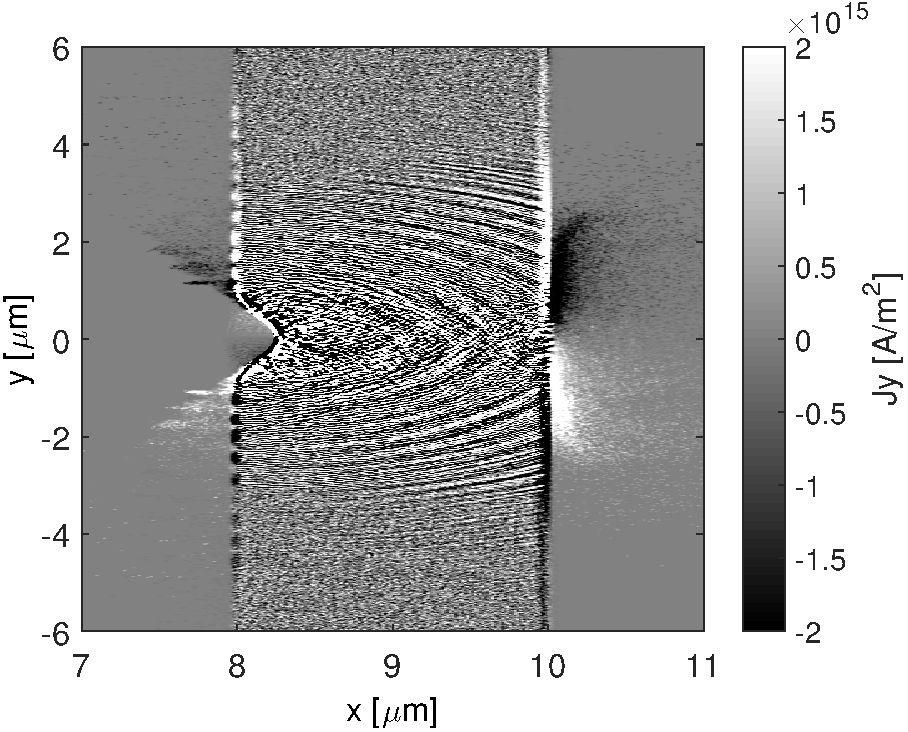
\includegraphics[width=0.45\linewidth]{./img/results/i1e21/05/jy.pdf}}}
	\sidesubfloat[]{{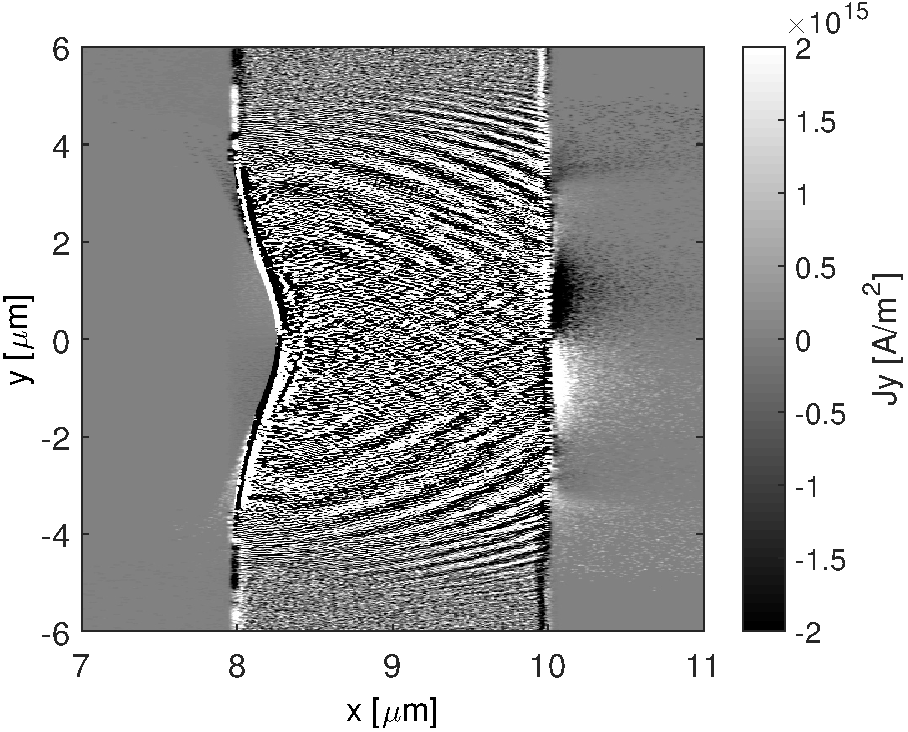
\includegraphics[width=0.45\linewidth]{./img/results/i1e21/2/jy.pdf}}}\\[2mm]
	\caption{Perpendicular component of the current density $ J_{y} $ at the time $ t = 100 \ \mathrm{fs} $ for the case of simulations with the laser intensity $ I = 10^{21} \ \mathrm{W/cm^2} $ and with the beam waist \textbf{(a)} $ w_0 = 0.5 \ \mu\mathrm{m} $, \textbf{(b)} $ w_0 = 2.0 \ \mu\mathrm{m} $. The color scale is saturated to demonstrate the features of the transverse return current. The real current density in the focal region is much higher.}
	\label{fig:18}
\end{figure}

\floatsetup[figure]{style=plain, subcapbesideposition=top}
\begin{figure}[h!]
	\centering
	\sidesubfloat[]{{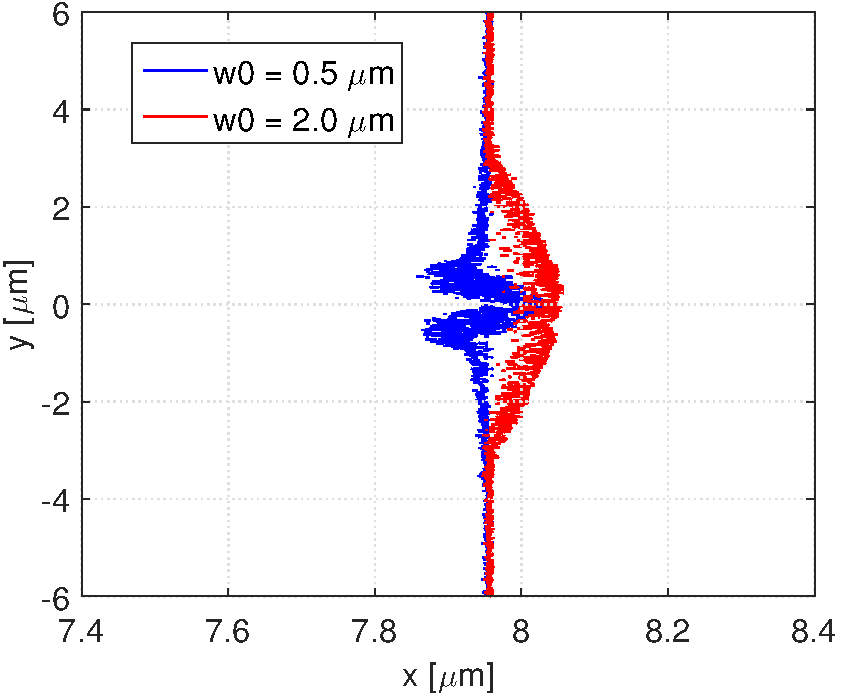
\includegraphics[width=0.445\linewidth]{./img/results/i1e20/dens.pdf}}}
	\hspace{1mm}
	\sidesubfloat[]{{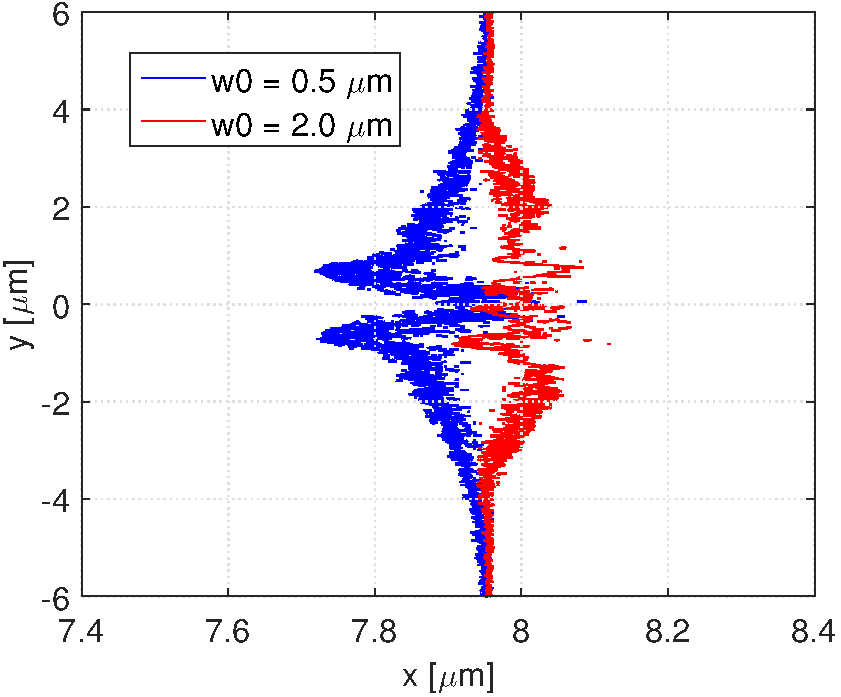
\includegraphics[width=0.445\linewidth]{./img/results/i1e21/dens.pdf}}}
	\caption{A contour lines of ion critical density for two different beam waists at the time $ t = 100 \ \mathrm{fs} $ for the case of simulations with the laser intensity \textbf{(a)} $ I = 10^{20} \ \mathrm{W/cm^2} $ and \textbf{(b)} $ I = 10^{21} \ \mathrm{W/cm^2} $.}
	\label{fig:15}
\end{figure}

\floatsetup[figure]{style=plain, subcapbesideposition=top}
\begin{figure}[h!]
	\centering
	\sidesubfloat[]{{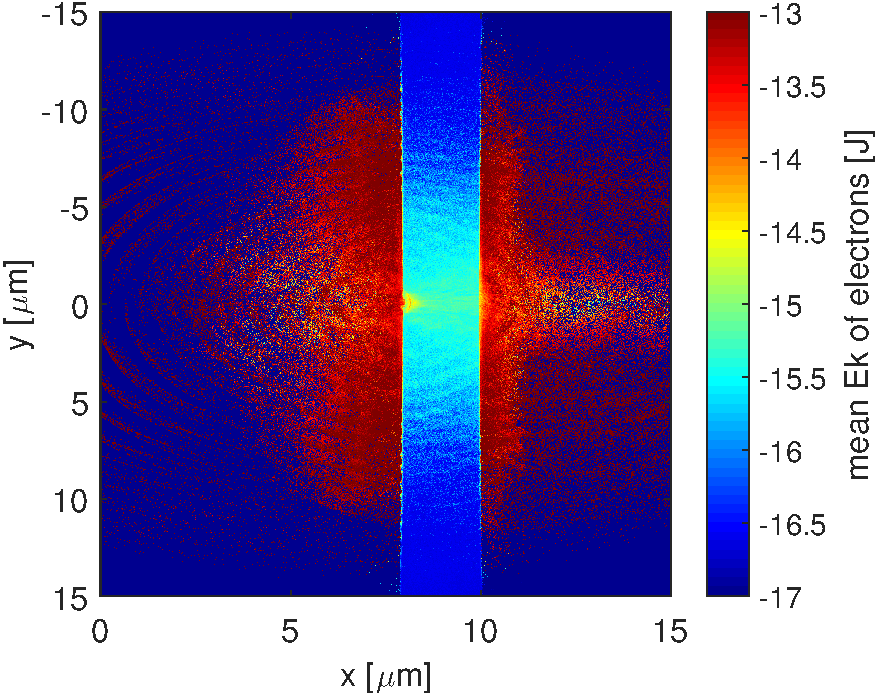
\includegraphics[width=0.45\linewidth]{./img/results/i1e20/05/ekbar.pdf}}}
	\sidesubfloat[]{{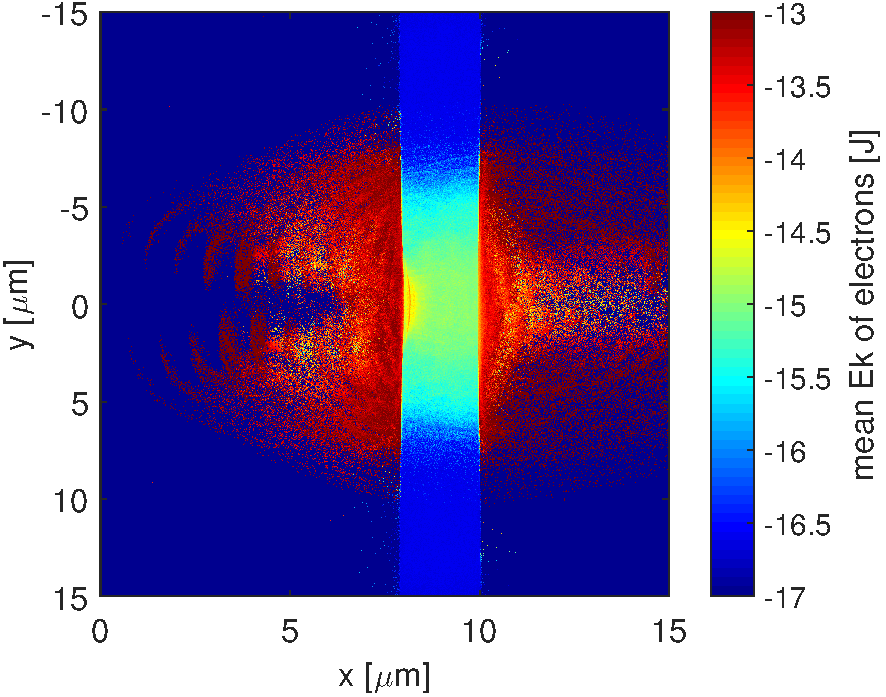
\includegraphics[width=0.45\linewidth]{./img/results/i1e20/2/ekbar.pdf}}}\\[2mm]
	\sidesubfloat[]{{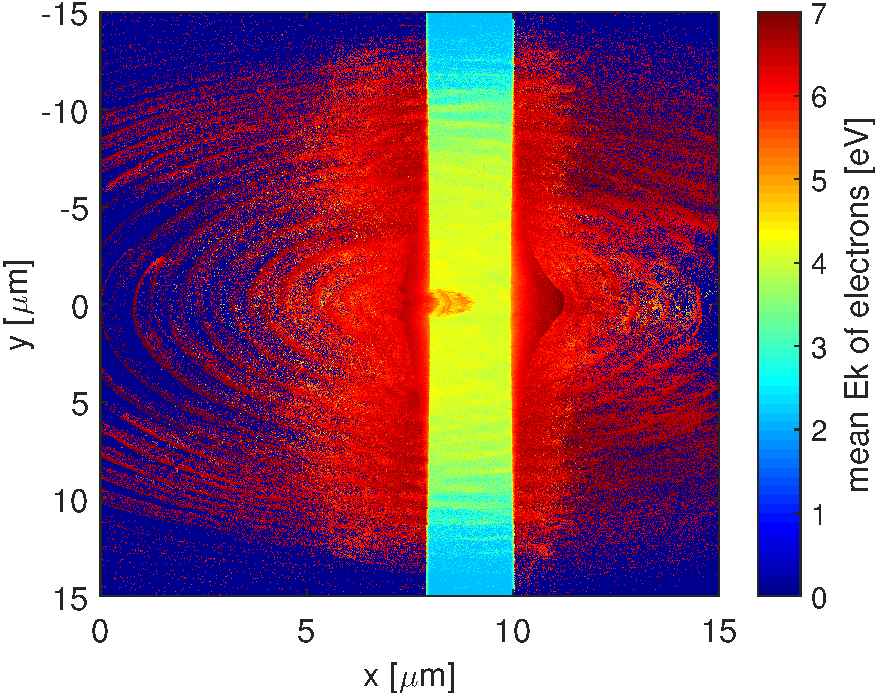
\includegraphics[width=0.45\linewidth]{./img/results/i1e21/05/ekbar.pdf}}}
	\sidesubfloat[]{{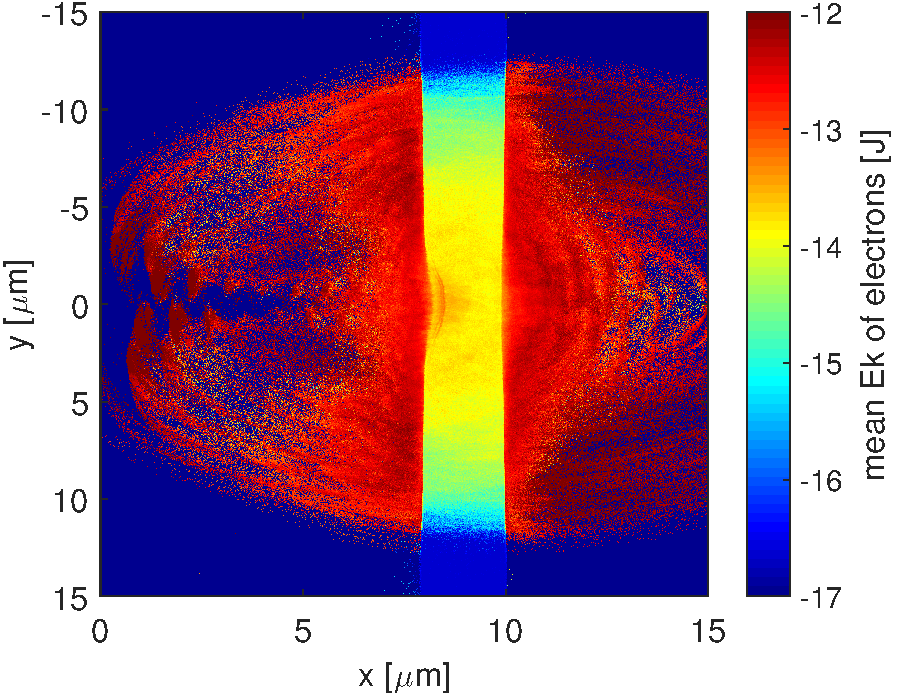
\includegraphics[width=0.45\linewidth]{./img/results/i1e21/2/ekbar.pdf}}}
	\caption{The spatial distribution of the mean kinetic energy of electrons at the time $ t = 120 \ \mathrm{fs} $ for the case of simulations with the laser intensity $ I = 10^{20} \ \mathrm{W/cm^2} $ and with the beam waist \textbf{(a)} $ w_0 = 0.5 \ \mu\mathrm{m} $, \textbf{(b)} $ w_0 = 2.0 \ \mu\mathrm{m} $ and for the case of simulations with the laser intensity $ I = 10^{21} \ \mathrm{W/cm^2} $ and with the beam waist \textbf{(c)} $ w_0 = 0.5 \ \mu\mathrm{m} $, \textbf{(d)} $ w_0 = 2.0 \ \mu\mathrm{m} $. The color scales are logarithmic and saturated.}
	\label{fig:16}
\end{figure}

The perpendicular component of the current density at the time $ t = 100 \ \mathrm{fs} $ is shown in the fig. \ref{fig:18}. In the case of $ w_0 = 0.5 \ \mu\mathrm{m} $ (fig. \ref{fig:18}-a), one may register the electric current caused by the electrons ejected into vacuum at the front side. The charge unbalance is then compensated by the electric current along the front surface of the target and this might be the reason, why there is more electrons with the trajectories of the first type in this case. The fig. \ref{fig:18} also indicates a different shape of the target deformed during the hole boring phase. Therefore, one may be interested in contour lines of ion critical density that are shown in the fig. \ref{fig:15}. Notice that in the case of $ w_0 = 0.5 \ \mu\mathrm{m} $, the plasma in the vicinity of incoming laser beam expands rapidly due to the space charge induced by electrons ejected into vacuum (marked by blue lines in the fig. \ref{fig:15}-a, \ref{fig:15}-b). It means that the absorption processes which take place when the laser pulse is obliquely incident on a plasma density gradient (such as resonance absorption or vacuum heating) may also significantly contribute to the overall laser energy absorption (table \ref{table:2}), e.g. the incidence angles for the laser intensity $ I = 10^{21} \ \mathrm{W/cm^2} $ are about $ 20^{\circ} $ and $ 1.5^{\circ} $ for $ w_0 = 0.5 \ \mu\mathrm{m} $ and $ w_0 = 2.0 \ \mu\mathrm{m} $, respectively.

\floatsetup[figure]{style=plain, subcapbesideposition=top}
\begin{figure}[h!]
	\centering
	\sidesubfloat[]{{\includegraphics[width=0.45\linewidth]{./img/results/i1e20/05/abs_ex.pdf}}}
	\sidesubfloat[]{{\includegraphics[width=0.45\linewidth]{./img/results/i1e20/2/abs_ex.pdf}}}\\[2mm]
	\sidesubfloat[]{{\includegraphics[width=0.45\linewidth]{./img/results/i1e21/05/abs_ex.pdf}}}
	\sidesubfloat[]{{\includegraphics[width=0.45\linewidth]{./img/results/i1e21/2/abs_ex.pdf}}}
	\caption{Longitudinal component of the electric field ($ E_{x} $) at the time $ t = 120 \ \mathrm{fs} $ for the case of simulations with the laser intensity $ I = 10^{20} \ \mathrm{W/cm^2} $ and with the beam waist \textbf{(a)} $ w_0 = 0.5 \ \mu\mathrm{m} $, \textbf{(b)} $ w_0 = 2.0 \ \mu\mathrm{m} $ and for the case of simulations with the laser intensity $ I = 10^{21} \ \mathrm{W/cm^2} $ and with the beam waist \textbf{(c)} $ w_0 = 0.5 \ \mu\mathrm{m} $, \textbf{(d)} $ w_0 = 2.0 \ \mu\mathrm{m} $. Note that in the case of $ w_0 = 2.0 \ \mu\mathrm{m} $, the color scales are saturated.}
	\label{fig:20}
\end{figure}

\floatsetup[figure]{style=plain, subcapbesideposition=top}
\begin{figure}[h!]
	\centering
	\sidesubfloat[]{{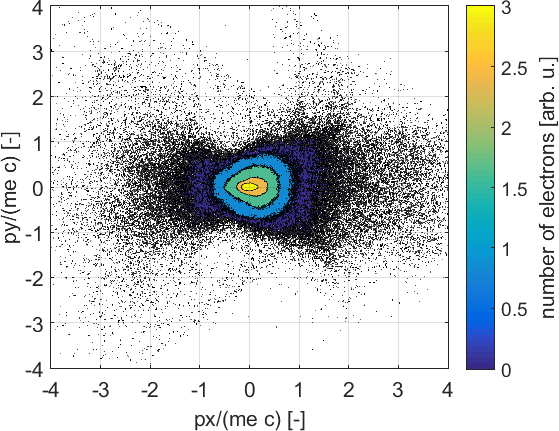
\includegraphics[width=0.45\linewidth]{./img/results/i1e20/05/px_py_final.png}}}
	\sidesubfloat[]{{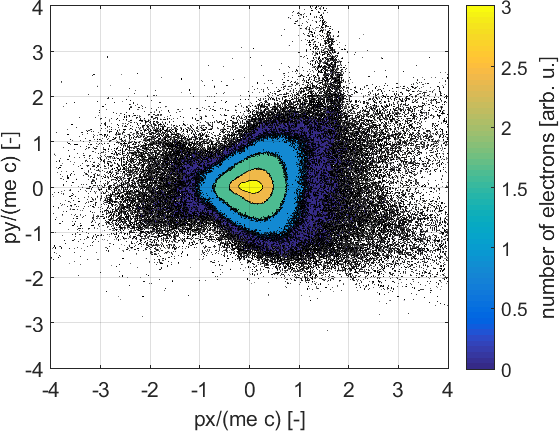
\includegraphics[width=0.45\linewidth]{./img/results/i1e20/2/px_py_final.png}}}\\
	\sidesubfloat[]{{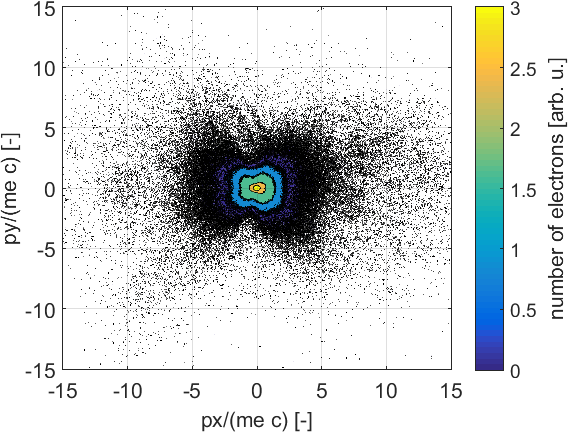
\includegraphics[width=0.45\linewidth]{./img/results/i1e21/05/px_py_final.png}}}
	\sidesubfloat[]{{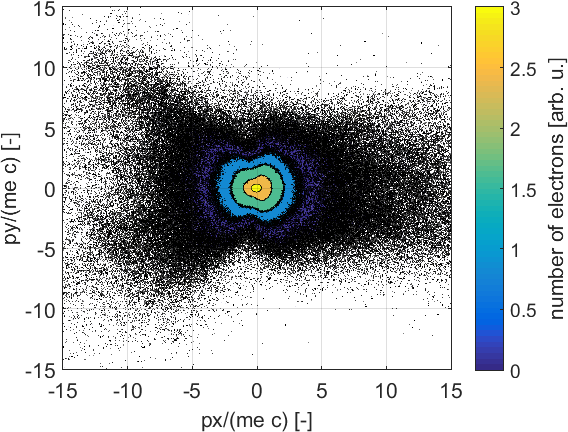
\includegraphics[width=0.45\linewidth]{./img/results/i1e21/2/px_py_final.png}}}
	\caption{Phase space of the parallel ($ p_x $) and the perpendicular ($ p_y $) components of the momentum of all electrons in the simulation domain at the time $ t = 100 \ \mathrm{fs} $ for the case of simulations with the laser intensity $ I = 10^{20} \ \mathrm{W/cm^2} $ and with the beam waist \textbf{(a)} $ w_0 = 0.5 \ \mu\mathrm{m} $, \textbf{(b)} $ w_0 = 2.0 \ \mu\mathrm{m} $ and for the case of simulations with the laser intensity $ I = 10^{21} \ \mathrm{W/cm^2} $ and with the beam waist \textbf{(c)} $ w_0 = 0.5 \ \mu\mathrm{m} $, \textbf{(d)} $ w_0 = 2.0 \ \mu\mathrm{m} $. The color scales are logarithmic and the units are arbitrary, but the same for all sub-figures.}
	\label{fig:12}
\end{figure}

The spatial distribution of the mean kinetic energy of electrons at the time $ t = 120 \ \mathrm{fs} $ in a global view is shown in the fig. \ref{fig:16}. Again, one can clearly see that in the case of $ w_0 = 0.5 \ \mu\mathrm{m} $ (fig. \ref{fig:16}-a), hot electrons spread out in the transverse direction more quickly than in the case of $ w_0 = 2.0 \ \mu\mathrm{m} $ (fig. \ref{fig:16}-b). For the laser intensity $ I = 10^{21} \ \mathrm{W/cm^2} $, however, the difference is less noticeable (fig. \ref{fig:16}-c, \ref{fig:16}-d).

\floatsetup[figure]{style=plain, subcapbesideposition=top}
\begin{figure}[h!]
	\centering
	\sidesubfloat[]{{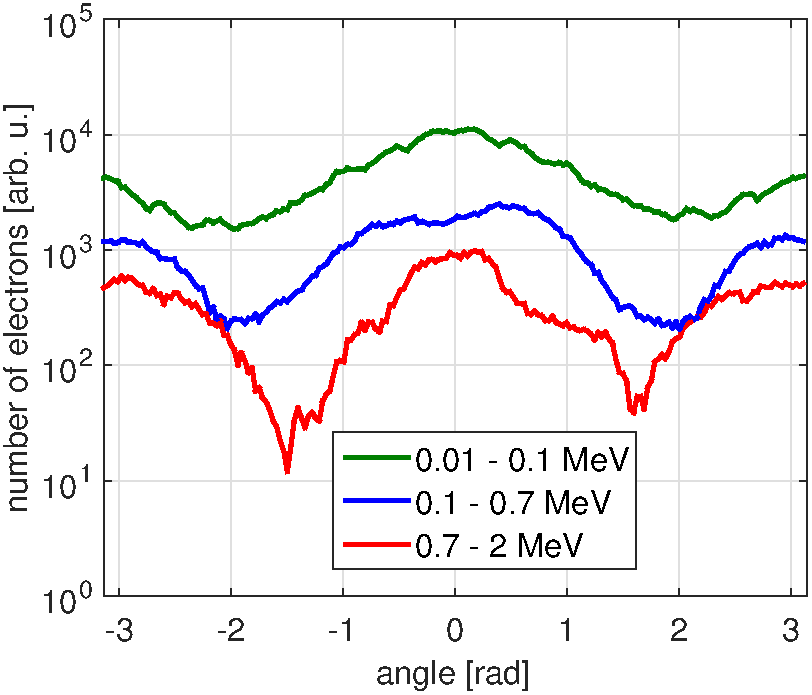
\includegraphics[width=0.445\linewidth]{./img/results/i1e20/05/angles.pdf}}}
	\hspace{1mm}
	\sidesubfloat[]{{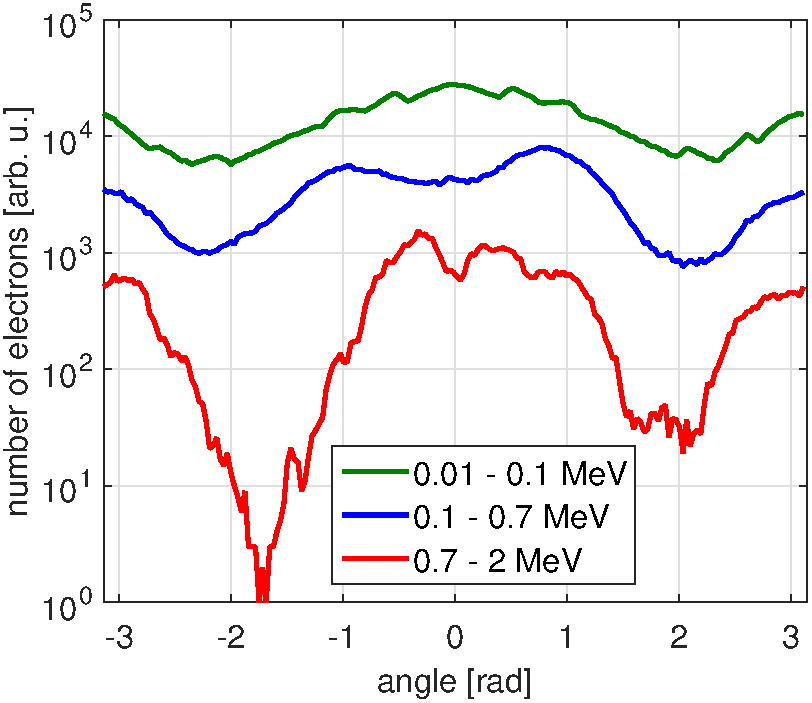
\includegraphics[width=0.445\linewidth]{./img/results/i1e20/2/angles.pdf}}}\\
	\sidesubfloat[]{{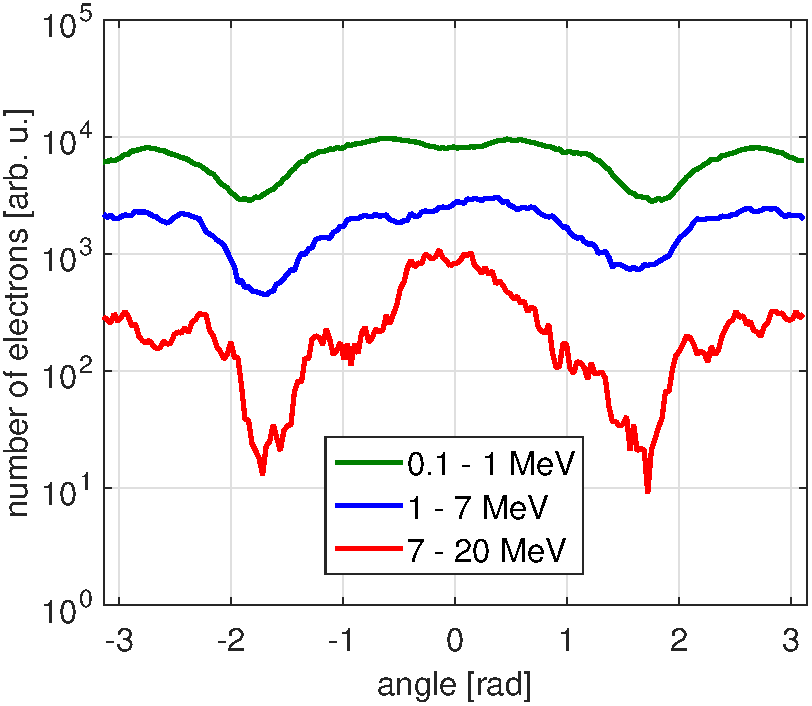
\includegraphics[width=0.445\linewidth]{./img/results/i1e21/05/angles.pdf}}}
	\hspace{1mm}
	\sidesubfloat[]{{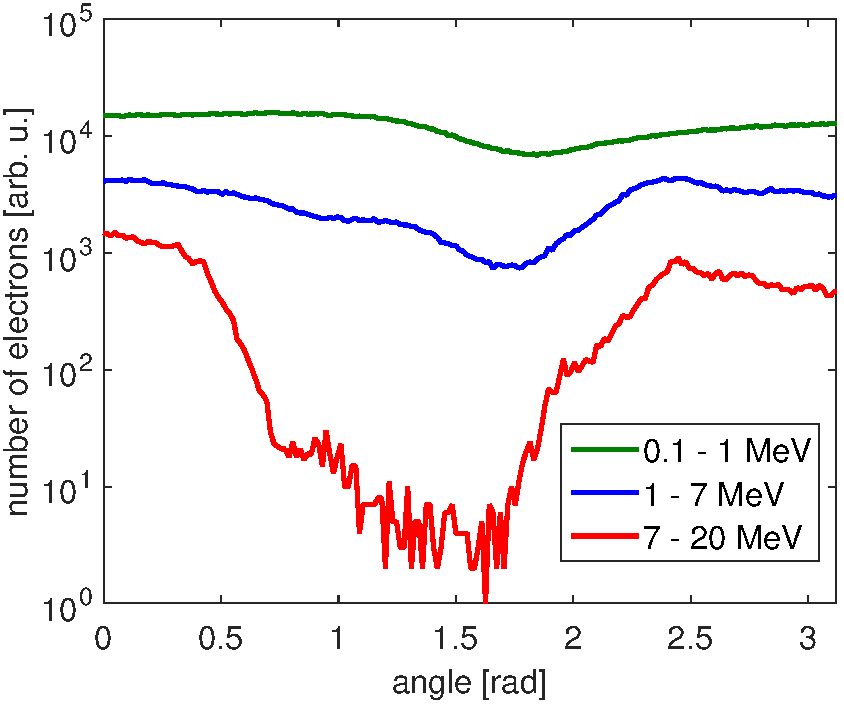
\includegraphics[width=0.445\linewidth]{./img/results/i1e21/2/angles.pdf}}}
	\caption{Angular distribution of electrons (the angle is measured with respect to the laser incidence direction) in the whole simulation domain at the time $ t = 100 \ \mathrm{fs} $ for the case of simulations with the laser intensity $ I = 10^{20} \ \mathrm{W/cm^2} $ and with the beam waist \textbf{(a)} $ w_0 = 0.5 \ \mu\mathrm{m} $, \textbf{(b)} $ w_0 = 2.0 \ \mu\mathrm{m} $ and for the case of simulations with the laser intensity $ I = 10^{21} \ \mathrm{W/cm^2} $ and with the beam waist \textbf{(c)} $ w_0 = 0.5 \ \mu\mathrm{m} $, \textbf{(d)} $ w_0 = 2.0 \ \mu\mathrm{m} $. The electrons are divided according to their kinetic energy into three separated intervals.}
	\label{fig:13}
\end{figure}

Additionally, the longitudinal component of the electric field in the simulation box at the time $ t = 120 \ \mathrm{fs} $ is demonstrated in the fig. \ref{fig:20}. Note that in the case of $ w_0 = 2.0 \ \mu\mathrm{m} $, the longitudinal electric field is slightly stronger, which is not observed in the fig. \ref{fig:20} due to the color saturation. As already mentioned, the hot electron energy is consequently transfered to ions faster. However, this is not the maximum longitudinal electric field, which occurs at $ t = 100 \ \mathrm{fs} $ and it is stronger for smaller spot size at lower intensity. As a result, the field decays faster for the case of $ w_0 = 0.5 \ \mu\mathrm{m} $ which is in agreement with higher divergence of hot electrons observed in this case. For the higher laser intensity the maximum longitudinal electric field is higher for the larger spot size so one cannot make the same conclusion about its faster decay. There is also a large difference between the shapes of the reflected laser light for both cases. While in the case of $ w_0 = 2.0 \ \mu\mathrm{m} $ (fig. \ref{fig:20}-b, \ref{fig:20}-d) the laser light is reflected in a relatively narrow beam, in the case of $ w_0 = 0.5 \ \mu\mathrm{m} $ (fig. \ref{fig:20}-a, \ref{fig:20}-c) the reflected light spreads radially outwards from the focal point. Nevertheless, divergence of the incident and the reflected laser beams are not much different.

\floatsetup[figure]{style=plain, subcapbesideposition=top}
\begin{figure}[h!]
	\centering
	\sidesubfloat[]{{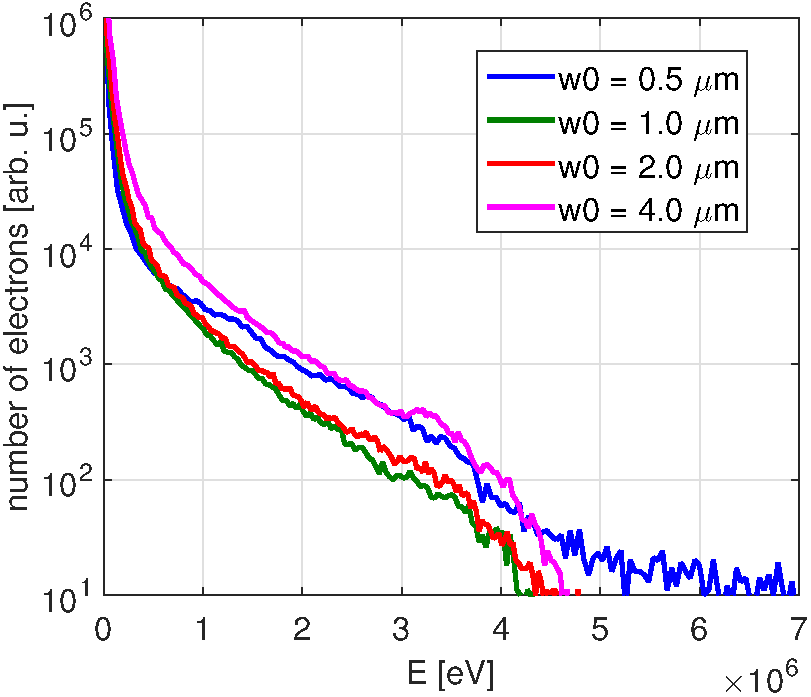
\includegraphics[width=0.435\linewidth]{./img/results/i1e20/dist_e.pdf}}}
	\hspace{1mm}
	\sidesubfloat[]{{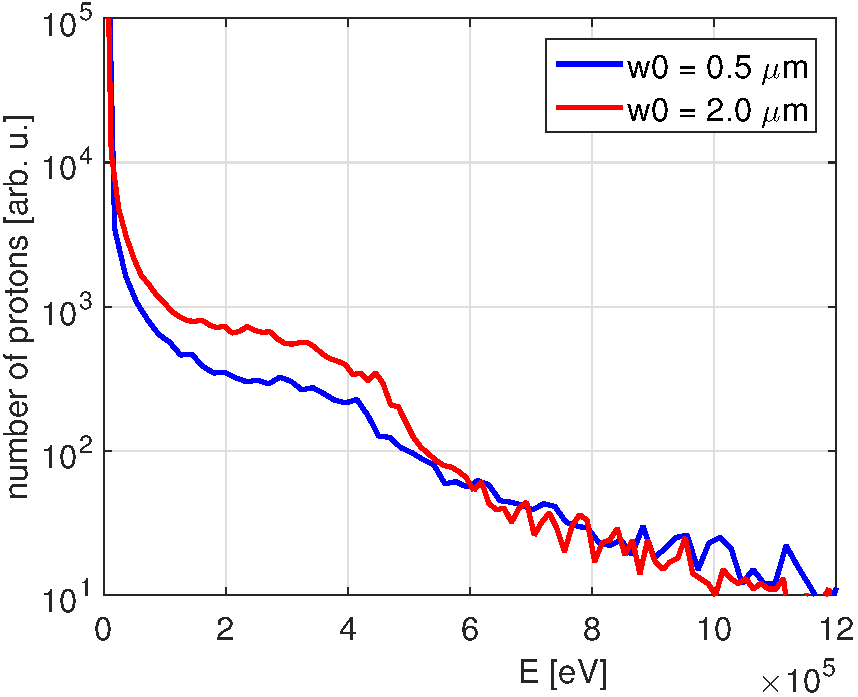
\includegraphics[width=0.435\linewidth]{./img/results/i1e20/dist_p.pdf}}}\\[1mm]
	\sidesubfloat[]{{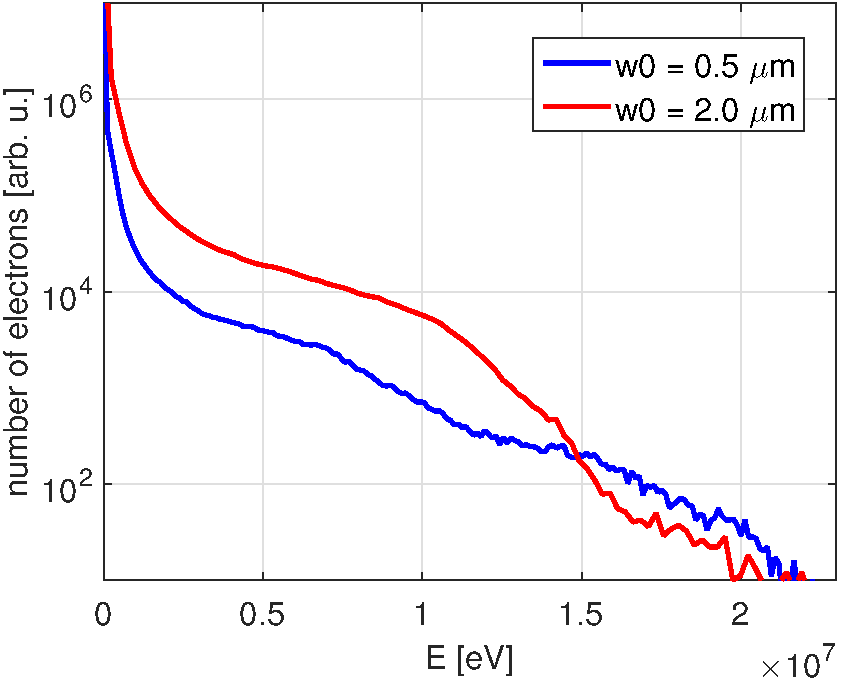
\includegraphics[width=0.435\linewidth]{./img/results/i1e21/dist_e.pdf}}}
	\hspace{1mm}
	\sidesubfloat[]{{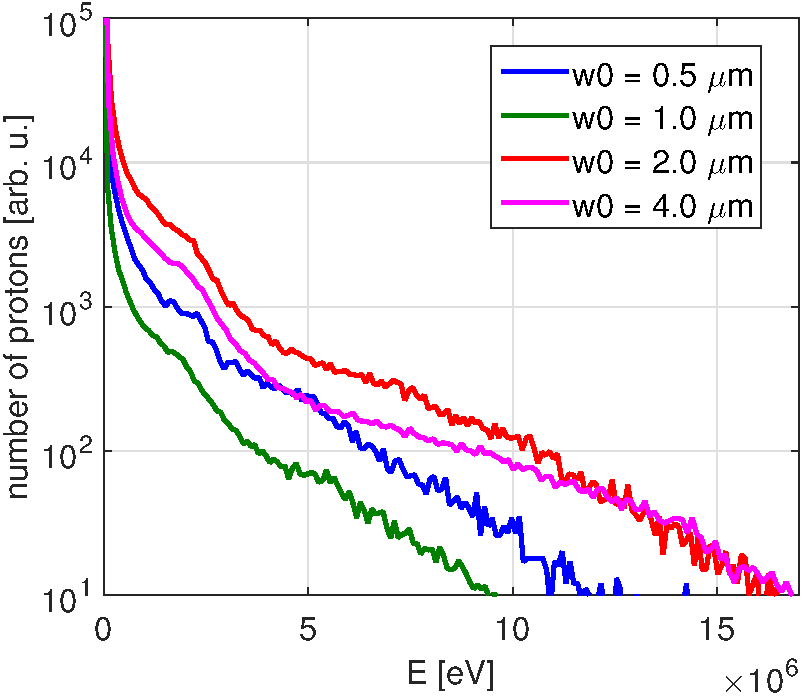
\includegraphics[width=0.435\linewidth]{./img/results/i1e21/dist_p.pdf}}}
	\caption{Electron energy distribution in the whole simulation domain for four different beam waists at the time $ t = 100 \ \mathrm{fs} $ for the case of simulations with the laser intensity \textbf{(a)} $ I = 10^{20} \ \mathrm{W/cm^2} $ and \textbf{(c)} $ I = 10^{21} \ \mathrm{W/cm^2} $. Ion energy distribution in the whole simulation domain for four different beam waists at the time $ t = 150 \ \mathrm{fs} $ for the case of simulations with the laser intensity \textbf{(b)} $ I = 10^{20} \ \mathrm{W/cm^2} $ and \textbf{(d)} $ I = 10^{21} \ \mathrm{W/cm^2} $.}
	\label{fig:14}
\end{figure}

The phase space of the parallel and the perpendicular components of the momentum of all electrons in the simulation domain at the time $ t = 100 \ \mathrm{fs} $ is shown in the fig. \ref{fig:12}. This might be particularly useful for determining the propagation direction of electrons. As one can clearly see, electrons propagate forward in a more collimated beam in the case of $ w_0 = 0.5 \ \mu\mathrm{m} $ (fig. \ref{fig:12}-a) than in the case of $ w_0 = 2.0 \ \mu\mathrm{m} $ (fig. \ref{fig:12}-b). Note that this would be in a contradiction with the previous observations. The fig. \ref{fig:12}, however, does not provide a complete information about the high-energy electrons. For the laser intensity $ I = 10^{21} \ \mathrm{W/cm^2} $, one cannot easily recognize differences in the shape of both electron distribution functions (fig. \ref{fig:12}-c, \ref{fig:12}-d).

The fig. \ref{fig:13} demonstrates the angular distribution of electrons in the whole simulation domain at the time $ t = 100 \ \mathrm{fs} $. It might be seen that in the case of $ w_0 = 0.5 \ \mu\mathrm{m} $, the lower-energy electrons (green and blue lines in the fig. \ref{fig:13}-a) propagate forward in a narrower beam than in the case of $ w_0 = 2.0 \ \mu\mathrm{m} $ (green and blue lines in the fig. \ref{fig:13}-b) which is in accordance with the fig. \ref{fig:12}. The divergence angle of the high-energy electrons propagating forward is almost identical for both cases (red line in the fig. \ref{fig:13}-a, \ref{fig:13}-b). However, in the case of $ w_0 = 0.5 \ \mu\mathrm{m} $, there is much more electrons spreading in the transverse direction (angle of $ \pm \pi/2 $) with respect to the incidence direction of the incoming laser pulse. Regarding the laser intensity $ I = 10^{21} \ \mathrm{W/cm^2} $, the angular distribution of lower-energy electrons is more isotropic (green and blue lines in the fig. \ref{fig:13}-c, \ref{fig:13}-d). The high-energy electrons propagate forward in a more collimated beam in the case of $ w_0 = 2.0 \ \mu\mathrm{m} $ (red line in the fig. \ref{fig:13}-d). However, in the case of $ w_0 = 0.5 \ \mu\mathrm{m} $ (red line in the fig. \ref{fig:13}-c), there is again larger amount of electrons spreading to the sides with respect to the incoming laser pulse.

The electron energy distribution functions at the time $ t = 100 \ \mathrm{fs} $ as well as the ion energy distributions at the time $ t = 150 \ \mathrm{fs} $ are shown in the fig. \ref{fig:14}. Apart from the case of $ w_0 = 0.5 \ \mu\mathrm{m} $, the high-energy tail of distribution functions has a similar slope which indicates the same hot electron temperatures (fig. \ref{fig:14}-a). In the case of $ w_0 = 0.5 \ \mu\mathrm{m} $, the temperature of hot electrons is significantly higher (blue line in the fig. \ref{fig:14}-a). Regarding the laser intensity $ I = 10^{21} \ \mathrm{W/cm^2} $, the energy distribution function of electrons in the case of $ w_0 = 0.5 \ \mu\mathrm{m} $ (blue line in the fig. \ref{fig:14}-c) is quantitatively different than the distribution functions for the other focal spot sizes. However, the energy distributions of hot electrons may be influenced by the TNSA process which already sets in (fig. \ref{fig:10}) or by thermalizing boundary conditions.

Concerning the maximum ion energies (fig. \ref{fig:14}-b, \ref{fig:14}-d), one can clearly see that they increase with the focal spot size. As already discussed, the electric field decays more slowly for larger spot sizes because it takes more time for hot electrons to spread transversally. Moreover, for the higher intensity, even the peak longitudinal electric field is higher. Therefore, in spite of the fact that the absorption is lower for larger spot size, ion acceleration efficiency is similar to the case of smaller spot size and the cut-off energy of ions is significantly higher.